%%%%%%%%%%%%%%%%%%%%%%%%%%%%%%%%%%%%%%%%%%%%%%%%%%%%%%%%%%%%%%%%
%%                                                            %%
%% latinProseComposition, Italian translation 2016.12 - 2017  %%
%%                                                            %%
%% From:  Henry Carr Pearson, Latin Prose Composition         %%
%%        (1903, New York, American Book Company)             %%
%%                                                            %%
%%    https://archive.org/details/latinprosecompo01peargoog   %%
%%                                                            %%
%% Translated by g.p.ciceri <gp.ciceri@gmail.com>             %%
%% ---------------------------------------------------------- %%
%% This translation is Licensed under                         %%
%% Creative Commons Attribution-ShareAlike 4.0 International  %%
%% https://creativecommons.org/licenses/by-sa/4.0/            %%
%%                                                            %%
%%%%%%%%%%%%%%%%%%%%%%%%%%%%%%%%%%%%%%%%%%%%%%%%%%%%%%%%%%%%%%%%

% āēīōū
% ăĕĭŏŭ




\documentclass[nols]{tufte-handout}

%\geometry{showframe} % display margins for debugging page layout

\usepackage{fontspec}
\usepackage{ifxetex}
\setmainfont[Path=./fonts/palatino-linotype/, ItalicFont=palai.ttf, BoldFont=palab.ttf]{pala.ttf}


% \defaultfontfeatures{Mapping=tex-text}
% \setromanfont[Path=./fonts/TeX-Gyre-Schola/,Mapping=tex-text]{TeX Gyre Schola}
% \setsansfont[Path=./fonts/TeX-Gyre-Heros/,Scale=MatchLowercase,Mapping=tex-text]{TeX Gyre Heros}
% \setmonofont[Path=./fonts/TeX-Gyre-Cursor/,Scale=MatchLowercase]{TeX Gyre Cursor}

\usepackage{lipsum}
\usepackage{url}
\usepackage{longtable}
\usepackage{stackengine}

\usepackage{graphicx} % allow embedded images
  \setkeys{Gin}{width=\linewidth,totalheight=\textheight,keepaspectratio}
  \graphicspath{{graphics/}} % set of paths to search for images
\usepackage{amsmath}  % extended mathematics
\usepackage{booktabs} % book-quality tables
\usepackage{units}    % non-stacked fractions and better unit spacing
\usepackage{multicol} % multiple column layout facilities
\usepackage{lipsum}   % filler text
\usepackage{fancyvrb} % extended verbatim environments
  \fvset{fontsize=\normalsize}% default font size for fancy-verbatim environments

% Standardize command font styles and environments
\newcommand{\doccmd}[1]{\texttt{\textbackslash#1}}% command name -- adds backslash automatically
\newcommand{\docopt}[1]{\ensuremath{\langle}\textrm{\textit{#1}}\ensuremath{\rangle}}% optional command argument
\newcommand{\docarg}[1]{\textrm{\textit{#1}}}% (required) command argument
\newcommand{\docenv}[1]{\textsf{#1}}% environment name
\newcommand{\docpkg}[1]{\texttt{#1}}% package name
\newcommand{\doccls}[1]{\texttt{#1}}% document class name
\newcommand{\docclsopt}[1]{\texttt{#1}}% document class option name
\newenvironment{docspec}{\begin{quote}\noindent}{\end{quote}}% command specification environment

% concetti morfosintattici
\usepackage{xspace} 
\newcommand{\noun}{\textsc{sostantivo}\xspace}
\newcommand{\nouns}{\textsc{sostantivi}\xspace}
\newcommand{\adject}{\textsc{aggettivo}\xspace}
\newcommand{\adjects}{\textsc{aggettivi}\xspace}
\newcommand{\gnumber}{\textsc{numero}\xspace}
\newcommand{\gnumbers}{\textsc{numeri}\xspace}
\newcommand{\gender}{\textsc{genere}\xspace}
\newcommand{\genders}{\textsc{generi}\xspace}
\newcommand{\gcase}{\textsc{caso}\xspace}
\newcommand{\gcases}{\textsc{casi}\xspace}
\newcommand{\tense}{\textsc{tempo}\xspace}
\newcommand{\mood}{\textsc{modo}\xspace}
\newcommand{\gverb}{\textsc{verbo}\xspace}
\newcommand{\gverbs}{\textsc{verbi}\xspace}
\newcommand{\adjective}{\textsc{aggettivo}\xspace}
\newcommand{\nom}{\textsc{nom}\xspace}
\newcommand{\gen}{\textsc{gen}\xspace}
\newcommand{\dat}{\textsc{dat}\xspace}
\newcommand{\acc}{\textsc{acc}\xspace}
\newcommand{\voc}{\textsc{voc}\xspace}
\newcommand{\abl}{\textsc{abl}\xspace}
\newcommand{\gexit}{\textsc{uscita}\xspace}
\newcommand{\gexits}{\textsc{uscite}\xspace}
\newcommand{\declinazione}{\textsc{declinazione}\xspace}
\newcommand{\masc}{\textsc{maschile}\xspace}
\newcommand{\femm}{\textsc{femminile}\xspace}
\newcommand{\neut}{\textsc{neutro}\xspace}

\newcommand{\indic}{\textsc{indicativo}\xspace}
\newcommand{\imper}{\textsc{imperativo}\xspace}
\newcommand{\gcong}{\textsc{congiuntivo}\xspace}
\newcommand{\ott}{\textsc{ottativo}\xspace}
\newcommand{\partic}{\textsc{participio}\xspace}
\newcommand{\infin}{\textsc{infinito}\xspace}

\newcommand{\pres}{\textsc{presente}\xspace}
\newcommand{\imperf}{\textsc{imperfetto}\xspace}
\newcommand{\aor}{\textsc{aoristo}\xspace}
\newcommand{\fut}{\textsc{futuro}\xspace}
\newcommand{\perf}{\textsc{perfetto}\xspace}
\newcommand{\pperf}{\textsc{piuccheperfetto}\xspace}

\newcommand{\sing}{\textsc{singolare}\xspace}
\newcommand{\plur}{\textsc{plurale}\xspace}
\newcommand{\dual}{\textsc{duale}\xspace}

\newcommand{\si}{\textsc{sing}\xspace}
\newcommand{\pl}{\textsc{plur}\xspace}
\newcommand{\du}{\textsc{dual}\xspace}

\newcommand{\att}{\textsc{attivo}\xspace}
\newcommand{\med}{\textsc{medio}\xspace}
\newcommand{\pass}{\textsc{passivo}\xspace}
\newcommand{\medpass}{\textsc{medio-passivo}\xspace}


% italianitudini
\renewcommand{\figurename}{Figura}
\renewcommand{\tablename}{Tabella}
\renewcommand{\contentsname}{Indice}

% fix per un qualche problema
\ifxetex
  \newcommand{\textls}[2][5]{%
    \begingroup\addfontfeatures{LetterSpace=#1}#2\endgroup
  }
  \renewcommand{\allcapsspacing}[1]{\textls[15]{#1}}
  \renewcommand{\smallcapsspacing}[1]{\textls[10]{#1}}
  \renewcommand{\allcaps}[1]{\textls[15]{\MakeTextUppercase{#1}}}
  \renewcommand{\smallcaps}[1]{\smallcapsspacing{\scshape\MakeTextLowercase{#1}}}
  \renewcommand{\textsc}[1]{\smallcapsspacing{\textsmallcaps{#1}}}
\fi

% too many float...
\extrafloats{100}

\title{Latin Prose Composition. Per scrivere in Latino. \newline Lezione I - La concordanza di nomi, aggettivi e verbi).}

\author[gpciceri]{a cura di Milagathòs: Milo's help to enjoy humanities\marginnote{\url{http://www.milagathos.com}}
}

\date{11 Gennajo 2017} % without \date command, current date is supplied


\begin{document}

\maketitle% this prints the handout title, author, and date

\begin{marginfigure}[-3.0cm]
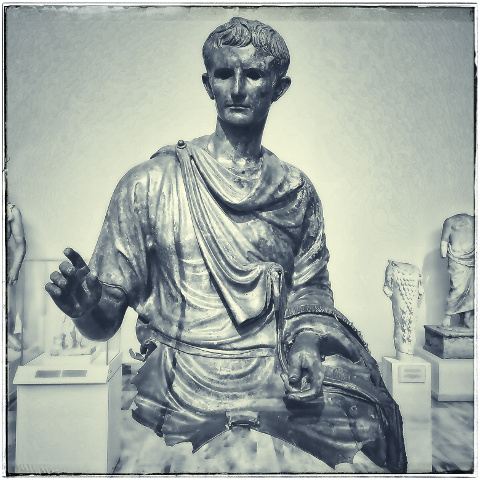
\includegraphics{smallthumb-lesson_I.jpeg}
\setfloatalignment{b}
\end{marginfigure}


\begin{abstract}
\noindent
Queste lezioni riprendono la prima parte del manuale di composizione latina di Pearson\cite{pearson1903}, del quale seguono la numerazione;
la struttura della lezione è piuttosto regolare: ad un sintetico \textsc{richiamo morfosintattico} fanno seguito delle \textsc{frasi di esempio},
vi sono poi \textsc{riferimenti al testo di grammatica} (qui sono riportati solo quelli al testo di Harkness\cite{harkness1898}, con relativa numerazione [H nnn.]) 
dove le regole grammaticali sono spiegate per esteso e, alla fine della lezione, 
un \textsc{esercizio di composizione in latino} - delle brevi frasi da tradurre.

\bigskip
\noindent
Lezione I: concordanza di nomi, aggettivi e verbi, vocabolario, esercizi.
\end{abstract}

%\printclassoptions

\newthought{1. Apposizione} Un nome in apposizione ad un altro nome concorda con esso nel \textit{caso}, e quanto possibile anche in \textit{genere} e \textit{numero}. 
\\
\vspace{0.5em}
\noindent \hangindent=1em \textbf{Servius rex,} \textit{il re Servo.} \\
\noindent \hangindent=1em \textbf{quattuor hic primum omen equos vidi,} \textit{qui vidi quattro cavalli, il primo auspicio.}

\newthought{2.} Un nome in apposizione ad un pronome o aggettivo possessivo (e con un altro nome) può essere in \textit{genitivo}, perché il possessivo implica il caso genitivo.
\\
\vspace{0.5em}
\noindent \hangindent=1em \textbf{nomen meum absentis,} \textit{il mio nome in mia assenza} (cioè \textit{il mio nome di assente})\\

\newthought{3.} Un nome in apposizione è spesso reso con un'espressione di tempo, causa, ecc.
\\
\vspace{0.5em}
\noindent \hangindent=1em \textbf{litteras Graecas senex didici,} \textit{imparai il Greco da vecchio}\\
 
\newthought{4.} Un nome in funzione di predicato è un nome connesso con il soggetto della frase da una voce del verbo essere (\textbf{sum})
o di un verbo similare (cioè \textbf{fio}, \textit{divenire;} 
\textbf{videor}, \textit{seem;} 
\textbf{maneo}, \textit{rimanere;} 
\textbf{creor}, \textit{essere eletto;}
\textbf{appellor}, \textit{essere chiamato;}
\textbf{habeor}, \textit{essere ritenuto}):
\\
\vspace{0.5em}
\noindent \hangindent=1em \textbf{Cicero orator fuit,} \textit{Cicerone era un oratore.}\\
\noindent \hangindent=1em \textbf{Numa creatus est rex,} \textit{Numa fu eletto re.}\\
\noindent \hangindent=1em \textbf{Orestem se esse dixit,} \textit{disse che era Oreste.}
 
\newthought{Concordanza dei Nomi, Sezioni 1-4.} vedi [H 393.] 1,5,6,8.

\newthought{5.} Un aggettivo che si riferisce a due o più nomi di norma concorda con il più vicino:
\\
\vspace{0.5em}
\noindent \hangindent=1em \textbf{pater tuus et mater,} \textit{tuo padre e tua madre.}

\newthought{6.} Un aggettivo in funzione di predicato (ad es. un participio in un tempo composto) è generalmente al \textit{plurale} 
quando modifica (cioè, si riferisce a) due o più soggetti al singolare; è al \textit{plurale} se i soggetti sono esseri viventi di 
generi diversi, al \textit{neutro} se i soggetti sono cose, esseri inanimati. Se i soggetti rappresentano sia esseri animati che inanimati,
non vi è regola fissata:
\\
\vspace{0.5em}
\noindent \hangindent=1em \textbf{pater sosorque occisi sunt,} \textit{il padre e lasorella furono uccisi.}\\
\noindent \hangindent=1em \textbf{labor voluptasque inter se sunt juncta,} \textit{il lavoro e il piacere sono collegati tra di loro.}

\newthought{7.} Talvolta un aggettivo o un participio non concordano con un nome secondo la regola grammaticale prevista, ma piuttosto a senso o secondo il genere naturale del nome:
\\
\vspace{0.5em}
\noindent \hangindent=1em \textbf{hominum milia sex perterriti,} \textit{sei migliaia di uomini furono (molto) spaventati.}

\newthought{Concordanza degli Aggettivi, Sezioni 5-7.} vedi [H 394., 395.].

\newthought{8.} Quando un verbo ha due o più soggetti al singolare, il verbo può essere \textit{(a) al plurale} o \textit{(b) al singolare, in accordo al soggetto più vicino al verbo}:
\\
\vspace{0.5em}
\noindent \hangindent=1em \textbf{pater et avus mortui sunt,} \textit{(suo) padre e (suo) nonno sono morti.}\\
\noindent \hangindent=1em \textbf{senatus populusque Romanus voluit,} \textit{il senato ed il popolo romano vollero.}

\newthought{9.} Un nome collettivo prende di norma il verbo al singolare, ma spesso viene usato il plurale quando si pensa agli \textit{individui}:
\\
\vspace{0.5em}
\noindent \hangindent=1em \textbf{senatus haec intellegit,} \textit{il senato è a conoscenza di ciò.}\\
\noindent \hangindent=1em \textbf{cum tanta multitudo lapides conicerent,} \textit{mentre una grande moltitudine stava gettando delle pietre.}

\newthought{10.} Quando i soggetti differiscono per \textit{persona}, il verbo concorda con la prima persona rispetto alla seconda, 
e con la seconda persona rispetto alla terza:
\\
\vspace{0.5em}
\noindent \hangindent=1em \textbf{si tu et Tullia valetis, ego et ciceri valemus} \textit{se Tullia e tu state bene, Cicerone e io stiamo bene.}

\newthought{Concordanza dei Verbi, Sezioni 8-10.} vedi [H 389., 392.].

\newthought{11. Tradurre in Latino:}
\textsc{1.}~Da ragazza, era considerata saggia. \quad
\textsc{2.}~Tu e io faremo questo. \quad
\textsc{3.}~Un parte dei soldativennero mandati in battaglia. \quad
\textsc{4.}~Tua sorella e tuo fratello sono arrivati. \quad
\textsc{5.}~Lo diedero a Cesare, il console. \quad
\textsc{6.}~Il ragazzo e (sua) sorella furono molto coraggiosi. \quad
\textsc{7.}~Udii del tuo coraggio\sidenote{\textbf{de} + \abl} da giovane. \quad
\textsc{8.}~Zelo e pazienza sono detti virtù. \quad
\textsc{9.}~Duemila uomini vennero mandati in città. \quad
\textsc{10.}~Una moltitudine di soldati erano sulle mura.


\begin{figure*}[!b]
  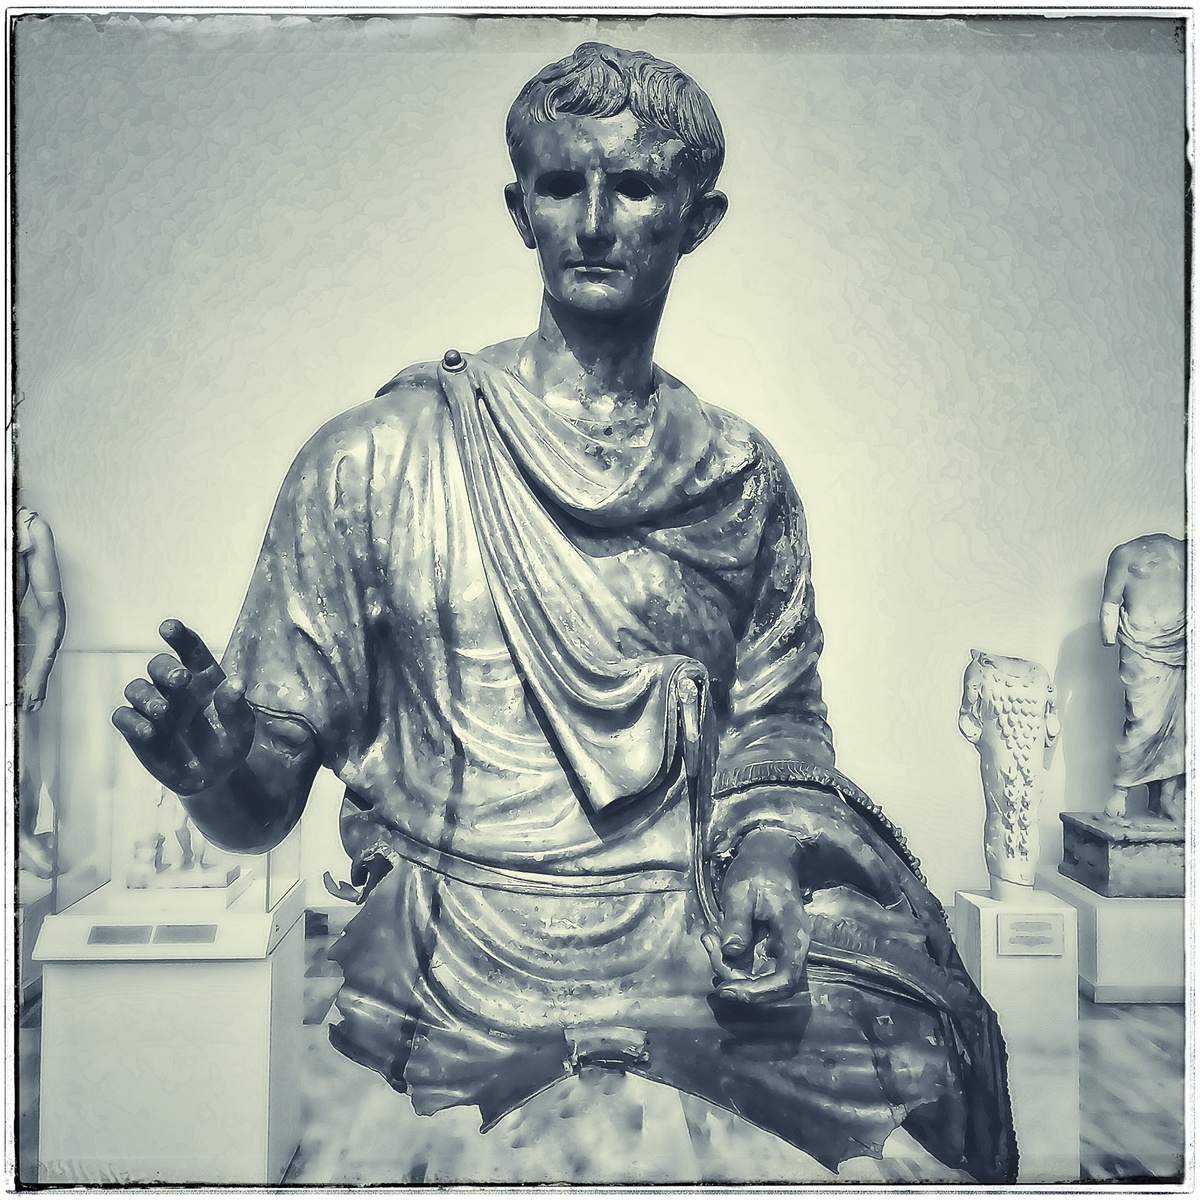
\includegraphics{thumb-lesson_I.jpeg}
  %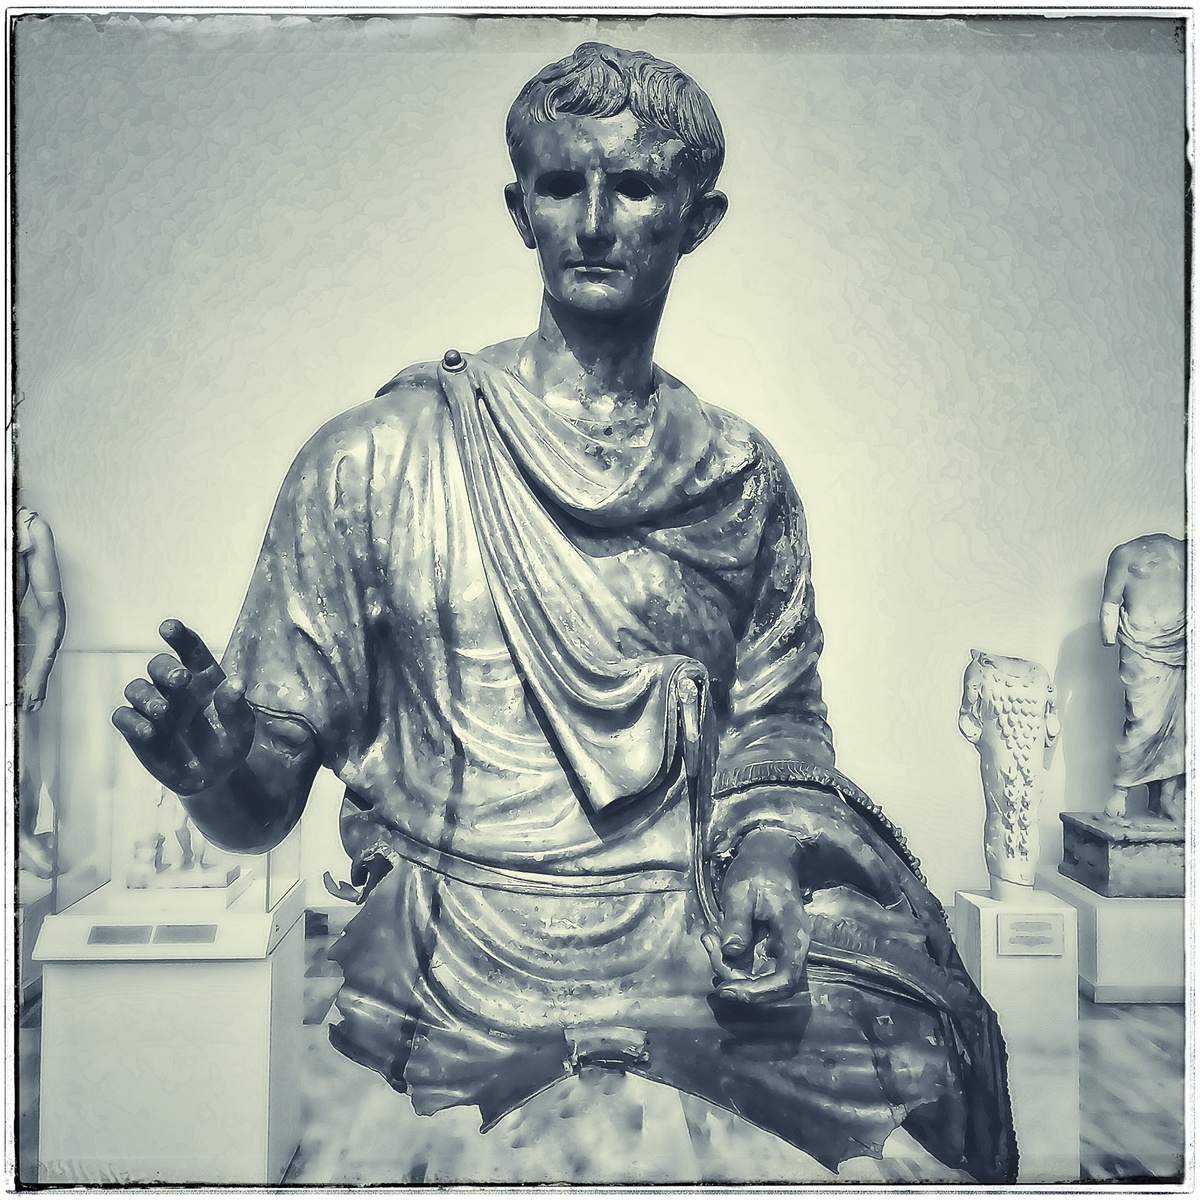
\includegraphics[width=0.5\linewidth]{thumb-lesson_I.jpeg}
  \caption{Museo Nazionale di Archeologia di Atene}
  \label{fig:textfig}
  %\zsavepos{pos:textfig}
  %\setfloatalignment{b}
\end{figure*}

 

\nobibliography{latinBiblio}
\bibliographystyle{alpha}


\end{document}
